\section{Vektorer i planen}
\noindent Vi er nu kommet til kursets sidste emner, som omhandler vektorer. En vektor er defineret ved at den har en længde og en retning, ofte tegnet som en pil (se Figur~\ref{fig:vec2d1et} hvor $\vec{u},\vec{v},\vec{w}$ er vektorer). Da vi kun er interesseret i en vektors længde og retning har vi at vektorerne $\vec{u}$ og $\vec{v}$ i Figur~\ref{fig:vec2d1et} er ens, da de har samme længde og samme retning, selvom de ikke er bestemt af de samme punkter. 

\begin{figure}[h!]
\centering
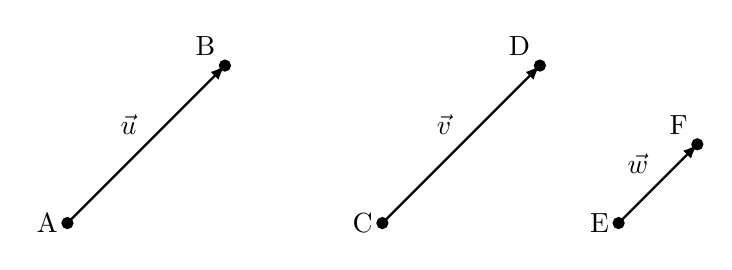
\begin{tikzpicture}
\coordinate (A) at (2,2);
\coordinate (B) at (4,4);

\draw [fill=black] (A) circle (2pt) node [left] {A};
\draw [fill=black] (B) circle (2pt) node [above left] {B};

\node[above left] at (3,3) {$\vec{u}$};

\draw [-latex, black, thick] (A) -- (B);

\coordinate (C) at (6,2);
\coordinate (D) at (8,4);

\draw [fill=black] (C) circle (2pt) node [left] {C};
\draw [fill=black] (D) circle (2pt) node [above left] {D};

\node[above left] at (7,3) {$\vec{v}$};

\draw [-latex, black, thick] (C) -- (D);

\coordinate (E) at (9,2);
\coordinate (F) at (10,3);

\draw [fill=black] (E) circle (2pt) node [left] {E};
\draw [fill=black] (F) circle (2pt) node [above left] {F};

\node[above left] at (9.5,2.5) {$\vec{w}$};

\draw [-latex, black, thick] (E) -- (F);

\end{tikzpicture}
\caption{Vektorer.}
\label{fig:vec2d1et}
\end{figure}

Vi vil starte ud med at studere 2-dimensionelle vektorer, som vi kan tænke på som værende punkter i et 2-dimensionalt koordinatsystem. Vi noterer en sådan vektor ved
\begin{align*}
\vec{v}=\begin{bmatrix}
x \\
y
\end{bmatrix}.
\end{align*}
\paragraph*{Regneregler:}
Lad $\vec{u} = \begin{bmatrix} x_1 \\ y_1 \end{bmatrix}$ og $\vec{v} = \begin{bmatrix} x_2 \\ y_2 \end{bmatrix}$, så har vi har følgende regneregler for vektorer.
\begin{enumerate}
\item $\displaystyle \vec{u} \pm \vec{v} = \begin{bmatrix} x_1 \\ y_1 \end{bmatrix} \pm \begin{bmatrix} x_2 \\ y_2 \end{bmatrix} = \begin{bmatrix} x_1 \pm x_2 \\ y_1 \pm y_2 \end{bmatrix} $.
\item $\displaystyle c \vec{u} = c  \begin{bmatrix} x_1 \\y_1 \end{bmatrix} = \begin{bmatrix} cx_1 \\ c y_1 \end{bmatrix}$, hvis $c \in \mathbb{R}$.
\item Længden af $\vec{u}$ noteres $\Vert \vec{u} \Vert$ og er givet ved $\displaystyle \Vert u \Vert = \sqrt{x_1^2+y_1^2}$
\end{enumerate}
For en illustration af hvad det vil sige at lægge to vektorer sammen og trække to vektorer fra hinanden se Figur~\ref{fig:vec2d1to} og~\ref{fig:vec2d1tre}. Bemærk, at hvis man ganger en vektor med en tal, så forlænger (forkorter) man vektoren med tallet og hvis tallet er negativ så ændrer også retningen, så vektoren går i den modsatte retning.
\begin{figure}[!htbp]
\begin{minipage}{0.49\textwidth}
\centering
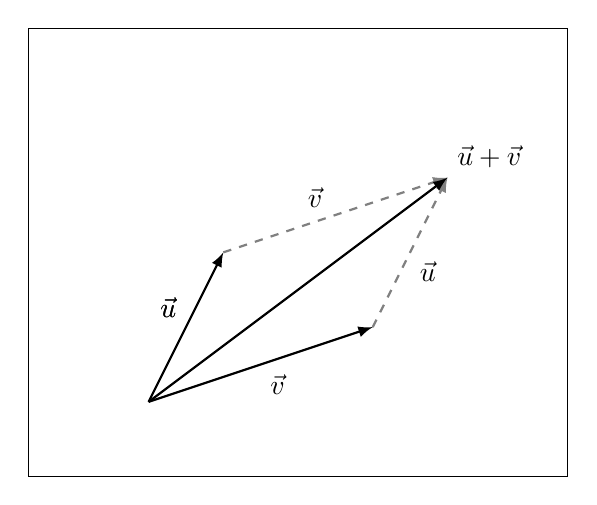
\begin{tikzpicture}
\begin{axis}[xmin=-1,xmax=5,ymin=-1,ymax=5,ticks=none, axis equal]
\coordinate (A) at (axis cs:0,0);
\coordinate (B) at (axis cs:1,2);
\node[above left] at (axis cs:0.5,1) {$\vec{u}$};
\draw [-latex, black, thick] (A) -- (B);
\coordinate (C) at (axis cs:3,1);
\node[below right] at (axis cs:1.5,0.5) {$\vec{v}$};
\draw [-latex, black, thick] (A) -- (C);
\coordinate (D) at (axis cs:4,3);
\node[above left] at (axis cs:0.5,1) {$\vec{u}$};
\draw [-latex, gray, thick,dashed] (B) -- (D);
\node[below right] at (axis cs:2,3) {$\vec{v}$};
\draw [-latex, gray, thick,dashed] (C) -- (D);
\node[below right] at (axis cs:3.5,2) {$\vec{u}$};
\node[above right] at (axis cs:4,3) {$\vec{u}+\vec{v}$};
\draw [-latex, black, thick] (A) -- (D);
\end{axis}
\end{tikzpicture}
\caption{$\vec{u}+\vec{v}$.}
\label{fig:vec2d1to}
\end{minipage}
\begin{minipage}{0.49\textwidth}
 \centering
\begin{tikzpicture}
\begin{axis}[xmin=-1,xmax=5,ymin=-1,ymax=5,ticks=none, axis equal]
\coordinate (A) at (axis cs:0,0);
\coordinate (B) at (axis cs:1,2);
\coordinate (C) at (axis cs:3,1);
\node[above left] at (axis cs:0.5,1) {$\vec{u}$};
\draw [-latex, black, thick] (A) -- (B);
\node[below right] at (axis cs:1.5,0.5) {$\vec{v}$};
\draw [-latex, black, thick] (A) -- (C);
\node[below right] at (axis cs:2,2) {$\vec{v}-\vec{u}$};
\draw [-latex, black, thick] (B) -- (C);
\end{axis}
\end{tikzpicture}
\caption{$\vec{v}-\vec{u}$.}
\label{fig:vec2d1tre}
\end{minipage}
\end{figure}

Hvis vi får givet to punkter i vores koordinatsystem $A=(x_1,y_1)$ og $B=(x_2,y_2)$ og vi gerne vil bestemme vektoren fra $A$ til $B$, så er den givet ved
\begin{align*}
\overrightarrow{AB}= \begin{bmatrix}
x_2-x_1 \\
y_2 - y_1
\end{bmatrix}.
\end{align*}

Det betyder at hvis $O$ er origo i vores koordinatsystem og $A=(x,y)$ så er vektoren fra origo til $A$ givet ved
\begin{align*}
\overrightarrow{OA}= \begin{bmatrix}x-0 \\y - 0\end{bmatrix}= \begin{bmatrix}x \\y\end{bmatrix}.
\end{align*}
Vi kalder vektoren der går fra origo til $A$ for stedvektoren til $A$. Da vi kun er interesseret i længden og retningen for en vektor og ikke de to punkter den går mellem, så vil vi som udgangspunkt tænke på en vektor som værende stedvektoren. Bemærk, at $\overrightarrow{OA}$ og $A$ har de samme koordinater, og derfor kan man både tænke på en vektor som et objekt med en længde og en retning, men også som et punkt i et koordinatsystem.

\paragraph*{Eksempler:}
\begin{enumerate}
\item Lad $\vec{u}= \begin{bmatrix} 3 \\ 2 \end{bmatrix}$ og $\vec{v}= \begin{bmatrix} 7 \\ 1 \end{bmatrix}$ og udregn $\vec{u}+\vec{v}$ og $\vec{v}-\vec{u}$:

Vi benytter regneregel $1$. og får
\begin{align*}
\vec{u} + \vec{v}&= \begin{bmatrix} 3 \\ 2 \end{bmatrix} + \begin{bmatrix} 7 \\ 1 \end{bmatrix} = \begin{bmatrix} 3+7 \\ 2+1 \end{bmatrix}  = \begin{bmatrix} 10 \\ 3 \end{bmatrix}. \\
\vec{v} - \vec{u}&= \begin{bmatrix} 7 \\ 1 \end{bmatrix} - \begin{bmatrix} 3 \\ 2 \end{bmatrix} = \begin{bmatrix} 7-3 \\ 1-2 \end{bmatrix}  = \begin{bmatrix} 4 \\ -1 \end{bmatrix}.
\end{align*}
\item Lad $\vec{u}= \begin{bmatrix} 1 \\ 2 \end{bmatrix}$ og udregn $3\vec{u}$:

Vi benytter regneregel $2$. og får
\begin{align*}
3\vec{u} = 3\begin{bmatrix} 1 \\ 2 \end{bmatrix} = \begin{bmatrix} 3\cdot 1 \\ 3 \cdot 2 \end{bmatrix}  = \begin{bmatrix} 3 \\ 6 \end{bmatrix}. 
\end{align*}
\item Lad $\vec{u}= \begin{bmatrix} 4 \\ 3 \end{bmatrix}$ og udregn $\norm{\vec{u}}$:

Vi benytter regneregel $3.$ og får
\begin{align*}
\norm{\vec{u}} = \sqrt{4^2+3^2} = \sqrt{16+9}= \sqrt{25}=5.
\end{align*}
\end{enumerate}

\paragraph*{Prikprodukt:}
Vi definerer prikproduktet mellem to vektorer $\vec{u} = \begin{bmatrix} x_1 \\ y_1 \end{bmatrix}$ og $\vec{v} = \begin{bmatrix} x_2 \\ y_2 \end{bmatrix}$ til at være
\begin{align}\label{eq:vec2d1prikprodukt}
\vec{u} \cdot \vec{v} =\begin{bmatrix} x_1 \\ y_1 \end{bmatrix} \cdot \begin{bmatrix} x_2 \\ y_2 \end{bmatrix} = x_1 x_2 + y_1  y_2.
\end{align}
Bemærk, at prikproduktet af to vektorer er et tal og ikke en vektor og at man ikke kan gange to vektorer sammen, man prikker dem sammen (så prikken mellem de to vektorer er ikke et gangetegn, men tegnet for et prikprodukt)!

Ved at benytte prikproduktet kan vi udregne vinklen $\theta$ mellem to vektorer $\vec{u}$ og $\vec{v}$ ved brug af formlen 
\begin{align}\label{eq:vec2d1vinkelvedprikprodukt}
\cos \theta = \frac{\vec{u} \cdot \vec{v}}{\norm{\vec{u}} \norm{\vec{v}}}.
\end{align}
Hvis prikproduktet $\vec{u} \cdot \vec{v}=0$, så har vi at 
\begin{align*}
\cos \theta = 0,
\end{align*}
hvilket betyder at $\theta$ er lig enten $\frac{\pi}{2}$ eller $\frac{3\pi}{2}$. Hvis vinklen mellem to vektorer er $\frac{\pi}{2}$ eller $\frac{3\pi}{2}$, så siger vi at de to vektorer er ortogonale (vinkelrette). Dermed har vi at 
\begin{align*}
\vec{u} \perp \vec{v} \qquad \textup{ hvis og kun hvis } \qquad \vec{u} \cdot \vec{v} = 0,
\end{align*}
hvor $\perp$ betyder at $\vec{u}$ og $\vec{v}$ er ortogonale.

Hvis man får givet en vektor $\vec{u} = \begin{bmatrix} x_1 \\ y_1 \end{bmatrix}$, og man gerne vil finde en vektor, som står ortogonalt på $\vec{u}$, så kan man gøre det ved at finde hatvektoren til $\vec{u}$, som er givet ved
\begin{align*}
\widehat{\vec{u}} = \begin{bmatrix}
-y_1 \\
x_1
\end{bmatrix}.
\end{align*}
I kommer selv i opgaveregningen til at vise at $\vec{u}$ og $\widehat{\vec{u}}$ faktisk er ortogonale.

\paragraph*{Determinant:}
Det næste vi vil betragte er determinanten af to vektorer. Hvis $\vec{u} = \begin{bmatrix} x_1 \\ y_1 \end{bmatrix}$ og $\vec{v} = \begin{bmatrix} x_2 \\ y_2 \end{bmatrix}$ så er determinanten af $\vec{u}$ og $\vec{v}$ givet ved
\begin{align}\label{eq:vec2d1determinant}
\det (\vec{u},\vec{v}) = \begin{vmatrix}
x_1 & x_2 \\
y_1 & y_2
\end{vmatrix}
=
x_1y_2 - x_2y_1.
\end{align}
Bemærk igen, at determinanten af to vektorer er et tal.

Ligesom ved prikproduktet kan vi også benytte determinanten mellem to vektorer $\vec{u}$ og $\vec{v}$ til at bestemme vinklen i mellem dem ud fra formlen
\begin{align}\label{eq:vec2d1vinkelveddeterminant}
\sin \theta = \frac{\det(\vec{u},\vec{v})}{\norm{\vec{u}}\norm{\vec{v}}}.
\end{align}
Hvis determinanten $\det(\vec{u}, \vec{v})=0$, så har vi at 
\begin{align*}
\sin \theta = 0,
\end{align*}
hvilket betyder at $\theta$ er lig enten $0$ eller $\pi$. Hvis vinklen mellem to vektorer er $0$ eller $\pi$, så siger vi at de to vektorer er parallelle. Dermed har vi at 
\begin{align*}
\vec{u} \parallel \vec{v} \qquad \textup{ hvis og kun hvis } \qquad \det(\vec{u}, \vec{v}) = 0,
\end{align*}
hvor $\parallel$ betyder at $\vec{u}$ og $\vec{v}$ er parallelle.

Derudover har vi, at absolutværdien af determinanten af $\vec{u}$ og $\vec{v}$ er lig med arealet af det parallelogram, der er udspændt af $\vec{u}$ og $\vec{v}$ (se Figur~\ref{fig:vec2d1to}), altså
\begin{align*}
A = \abs{\det( \vec{u},\vec{v} )},
\end{align*}
hvor $A$ er arealet af det udspændte parallelogram.

\paragraph*{Eksempler:}
\begin{enumerate}
\item Lad $\vec{u}= \begin{bmatrix} 3 \\ 2 \end{bmatrix}$ og $\vec{v}= \begin{bmatrix} 7 \\ 1 \end{bmatrix}$ og udregn $\vec{u}\cdot \vec{v}$ og $\det(\vec{u},\vec{v})$:

Vi benytter \eqref{eq:vec2d1prikprodukt} og \eqref{eq:vec2d1determinant} til at finde henholdsvis prikproduktet og determinanten
\begin{align*}
\vec{u}\cdot \vec{v} &=\begin{bmatrix} 3 \\ 2 \end{bmatrix}\cdot  \begin{bmatrix} 7 \\ 1 \end{bmatrix} = 3 \cdot 7 + 2 \cdot 1 = 21+2 = 23.\\
\det(\vec{u},\vec{v})&=\begin{vmatrix}
3 & 7 \\
2 & 1
\end{vmatrix}
=3 \cdot 1 - 2 \cdot 7 = 3-14=-11.
\end{align*}
\item Lad $\vec{u}= \begin{bmatrix} 0 \\ 1 \end{bmatrix}$ og $\vec{v}= \begin{bmatrix} 0 \\ -1 \end{bmatrix}$ og udregn vinklen mellem $\vec{u}$ og $\vec{v}$:

Vi kan udregne vinklen enten ved at benytte \eqref{eq:vec2d1vinkelvedprikprodukt} eller \eqref{eq:vec2d1vinkelveddeterminant}. Vi vælger at benytte \eqref{eq:vec2d1vinkelvedprikprodukt}, så vi finder først prikproduktet og normen af de to vektorer
\begin{align*}
\vec{u} \cdot \vec{v} &= \begin{bmatrix} 0 \\ 1 \end{bmatrix} \cdot \begin{bmatrix} 0 \\ -1 \end{bmatrix} = 0 \cdot 0 + 1 \cdot -1 = -1 \\
\norm{\vec{u}} &= \sqrt{0^2+1^2} = \sqrt{1}=1 \\
\norm{\vec{v}} &= \sqrt{0^2 + (-1)^2}=\sqrt{1}=1.
\end{align*}
Dermed har vi, at
\begin{align*}
\cos \theta = \frac{\vec{u} \cdot \vec{v}}{\norm{\vec{u}}\norm{\vec{v}}} = \frac{-1}{1 \cdot 1} = \frac{-1}{1} = -1.
\end{align*}
Dvs. at vinklen mellem $\vec{u}$ og $\vec{v}$ er den vinkel, der opfylder at $\cos \theta =-1$ og vi husker, at det gør $\theta = \pi$.
\item Lad $\vec{u}= \begin{bmatrix} 0 \\ 1 \end{bmatrix}$ og $\vec{v}= \begin{bmatrix} 1 \\ 0 \end{bmatrix}$ og bestem om $\vec{u}\perp \vec{v}$ eller $\vec{u} \parallel\vec{v}$:

Vi udregner prikproduktet og determinanten af de to vektorer
\begin{align*}
\vec{u} \cdot \vec{v} &= \begin{bmatrix} 0 \\ 1 \end{bmatrix}\cdot  \begin{bmatrix} 1 \\ 0 \end{bmatrix} = 0 \cdot 1 + 0 \cdot 1 = 0 \\
\det(\vec{u},\vec{v}) &= \begin{vmatrix}
1 & 0 \\
0 & 1
\end{vmatrix}
= 1 \cdot 1 - 0 \cdot 0 = 1.
\end{align*}
Da $\vec{u} \cdot \vec{v}=0$ men $\det(\vec{u},\vec{v})\neq 0$, har vi at $\vec{u}$ og $\vec{v}$ er ortogonale men ikke parallelle. Bemærk, at det eneste tidspunkt hvor to vektorer er både ortogonale og parallelle er hvis den ene af vektorerne er nulvektoren.
\end{enumerate}